%!TEX program = xelatex

\documentclass[compress]{beamer}
%--------------------------------------------------------------------------
% Common packages
%--------------------------------------------------------------------------

\definecolor{links}{HTML}{663000}
\hypersetup{colorlinks,linkcolor=,urlcolor=links}

\usepackage[english]{babel}
\usepackage{pgfpages} % required for notes on second screen
\usepackage{graphicx}

\usepackage{pdfpcnotes}

\usepackage{multicol}

\usepackage{tabularx,ragged2e}
\usepackage{booktabs}

\usetheme{hri}

% Display the navigation bullet even without subsections
\usepackage{remreset}% tiny package containing just the \@removefromreset command
\makeatletter
\@removefromreset{subsection}{section}
\makeatother
\setcounter{subsection}{1}

\makeatletter
\let\beamer@writeslidentry@miniframeson=\beamer@writeslidentry
\def\beamer@writeslidentry@miniframesoff{%
  \expandafter\beamer@ifempty\expandafter{\beamer@framestartpage}{}% does not happen normally
  {%else
    % removed \addtocontents commands
    \clearpage\beamer@notesactions%
  }
}
\newcommand*{\miniframeson}{\let\beamer@writeslidentry=\beamer@writeslidentry@miniframeson}
\newcommand*{\miniframesoff}{\let\beamer@writeslidentry=\beamer@writeslidentry@miniframesoff}
\makeatother



\newcommand{\source}[2]{{\tiny\it Source: \href{#1}{#2}}}

\usepackage[normalem]{ulem}

\usepackage{tikz}
\usetikzlibrary{intersections,arrows,shapes,calc,mindmap,backgrounds,positioning,svg.path}

\tikzset{box/.style={
            draw, 
            fill=blue!20,
            fill opacity=0.8,
            thick,
            inner sep=0pt,
            minimum size=1cm,
            transform shape
        },
        finalbox/.style={
            draw, 
            fill=orange,
            fill opacity=0.8,
            thick,
            inner sep=0pt,
            minimum size=1cm,
            transform shape
        },
        dot/.style={
            draw,
            circle,
            fill=red!20,
            inner sep=0pt,
            minimum size=1cm,
            transform shape
        },
        axis/.style={
            thick,
            gray,
            font=\small},
        every to/.style={
            >=latex,
            dashed,
            thick
        }
    }


\graphicspath{{figs/}{figs/anthropomorphism/}}

\title{Automatic Processing of Emotions}
\subtitle{AINT512}

\date{}
\author{Séverin Lemaignan}
\institute{Centre for Neural Systems and Robotics\\{\bf Plymouth University}}

\begin{document}

\miniframesoff

\licenseframe{github.com/severin-lemaignan/lecture-emotions}

\maketitle


\begin{frame}{This week}

This week, we are looking at the automatic processing of emotions:

    \begin{itemize}
        \item models of emotions
        \item action units
        \item emotion classification
        \item emotion generation
    \end{itemize}

\end{frame}

\miniframeson

\section{Models of emotion}

\begin{frame}{Paul Ekman and basic emotions}

\href{https://en.wikipedia.org/wiki/Paul_Ekman}{Paul Ekman}, a
psychologist, found that when shown facial expressions people across the
world all recognised six \textbf{basic emotions}.

    \only<1>{
    \begin{center}
        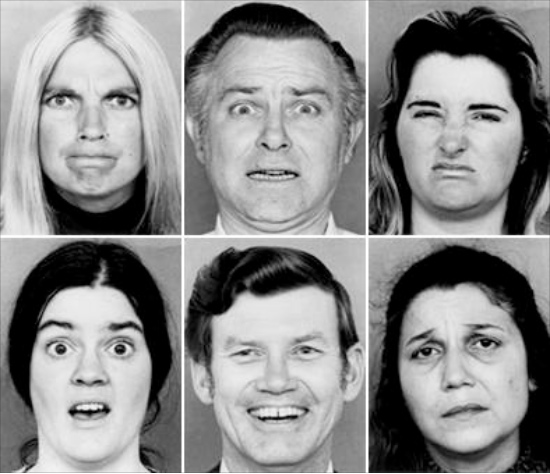
\includegraphics[width=0.55\linewidth]{ekman_6_basic_emotions}

        \source{http://emotionresearcher.com/}{emotionresearcher.com}
    \end{center}
}

\pause

\begin{center}
\textbf{Anger, disgust, fear, happiness, sadness and surprise}.
\end{center}

Some other emotion are less universally recognised, e.g.~contempt.

\pause 
In 1990 Ekman extended his list of basic emotion to include other
emotions: \emph{Amusement, contempt, contentment, embarrassment, excitement, guilt,
  pride in achievement, relief, satisfaction, sensory pleasure, and
    shame}


\end{frame}


\begin{frame}{Emotion and machines}

    \only<1-2>{
        {\bf Computer and robots should be able to read emotions}

    \begin{itemize}
        \item This is crucial in understanding the social world around the robot and
            responding appropriately.
        \item This has a large number of applications, e.g.
            \href{https://en.wikipedia.org/wiki/Sentiment_analysis}{sentiment
            analysis} to predict what the
            \href{http://arxiv.org/PS_cache/arxiv/pdf/1010/1010.3003v1.pdf}{stock
            market will do based on emotional content of tweets}.
    \end{itemize}

    \pause

    {\bf Should machines express emotions?}

    \begin{itemize}

        \item Due to the \href{https://en.wikipedia.org/wiki/The_Media_Equation}{\bf
            media equation} we cannot help attributing emotions to
            robots and other technology.
        \item As we expect machines to express emotions, it would be good as a robot
            designer to take control of the unconscious attribution of emotion by
            the user.
        \item + cf Serge's slides
    \end{itemize}

}
    \only<3>{
        {\bf Why would representing emotion be useful?}

    \begin{itemize}

        \item You can model the emotional state of the user and respond
            appropriately. For example, the user is bored, if the robot knows this
            it can do something to entertain the user.
        \item You can use a model to let the robot express emotions. For example,
            this can be used for ``emotion contagion''. If the robot is happy,
            this will influence how the user feels.
    \end{itemize}
}
\end{frame}

\begin{frame}{How to represent emotions?}

\only<1-4>{
    Several approaches (or {\bf models}):
}

\only<1-2>{
ON/OFF approach to basic emotions:

\begin{itemize}

\item Anger : ON/OFF
\item Disgust : ON/OFF
\item Fear : ON/OFF
\item Happiness : ON/OFF
\item Sadness : ON/OFF
\item Surprise : ON/OFF
\end{itemize}

Why is this a poor approach to representing emotion?

\pause

$\Rightarrow$ no representation of gradual emotions; all is just ``on'' or
``off''
}
\only<3-4>{


Gradual representation of emotion would be better:

\begin{itemize}

\item Anger : {[}0; 1{]}
\item Disgust : {[}0; 1{]}
\item Fear : {[}0; 1{]}
\item Happiness : {[}0; 1{]}
\item Sadness : {[}0; 1{]}
\item Surprise : {[}0; 1{]}
\end{itemize}

What is the problem with this representation?

\onslide<4>
$\Rightarrow$ can lead to contradicting emotion representation, for example
Happiness = 1 and Sadness = 1.
}


    \only<5>{
    $\Rightarrow$ continuous representations of emotions in space
}
\end{frame}

{
    \paper{Russell J. {\bf A circumplex model of affect} 1980}
\begin{frame}{Circumplex model}

Two-dimensional space (\textbf{arousal} and \textbf{valence} on x and y
dimensions)

\begin{itemize}

\item emotions are noted on circumference of the circle.
\item middle of circle (0,0) is \textbf{neutral}
\item the further from the centre, the stronger the emotion.
\end{itemize}

    \begin{center}
        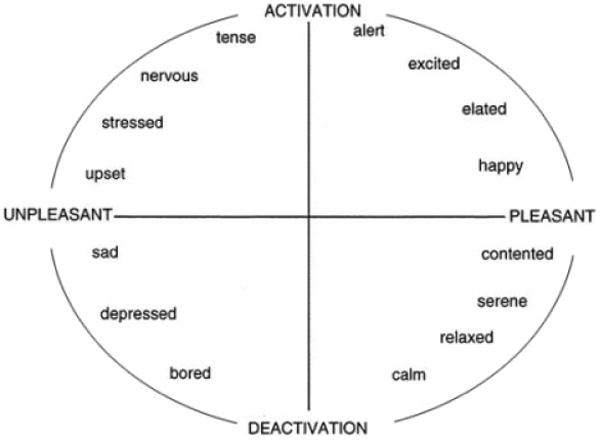
\includegraphics[width=0.55\linewidth]{circumplex}
        \source{http://www.ncbi.nlm.nih.gov/pmc/articles/PMC2367156/}{Posner
et al., 2005}
    \end{center}
\end{frame}
}

{
    \paper{Mollahosseini et al. {\bf Affectnet: A database for facial
    expression, valence, and arousal computing in the wild} 2017}
\begin{frame}{Circumplex model}
    \begin{center}
        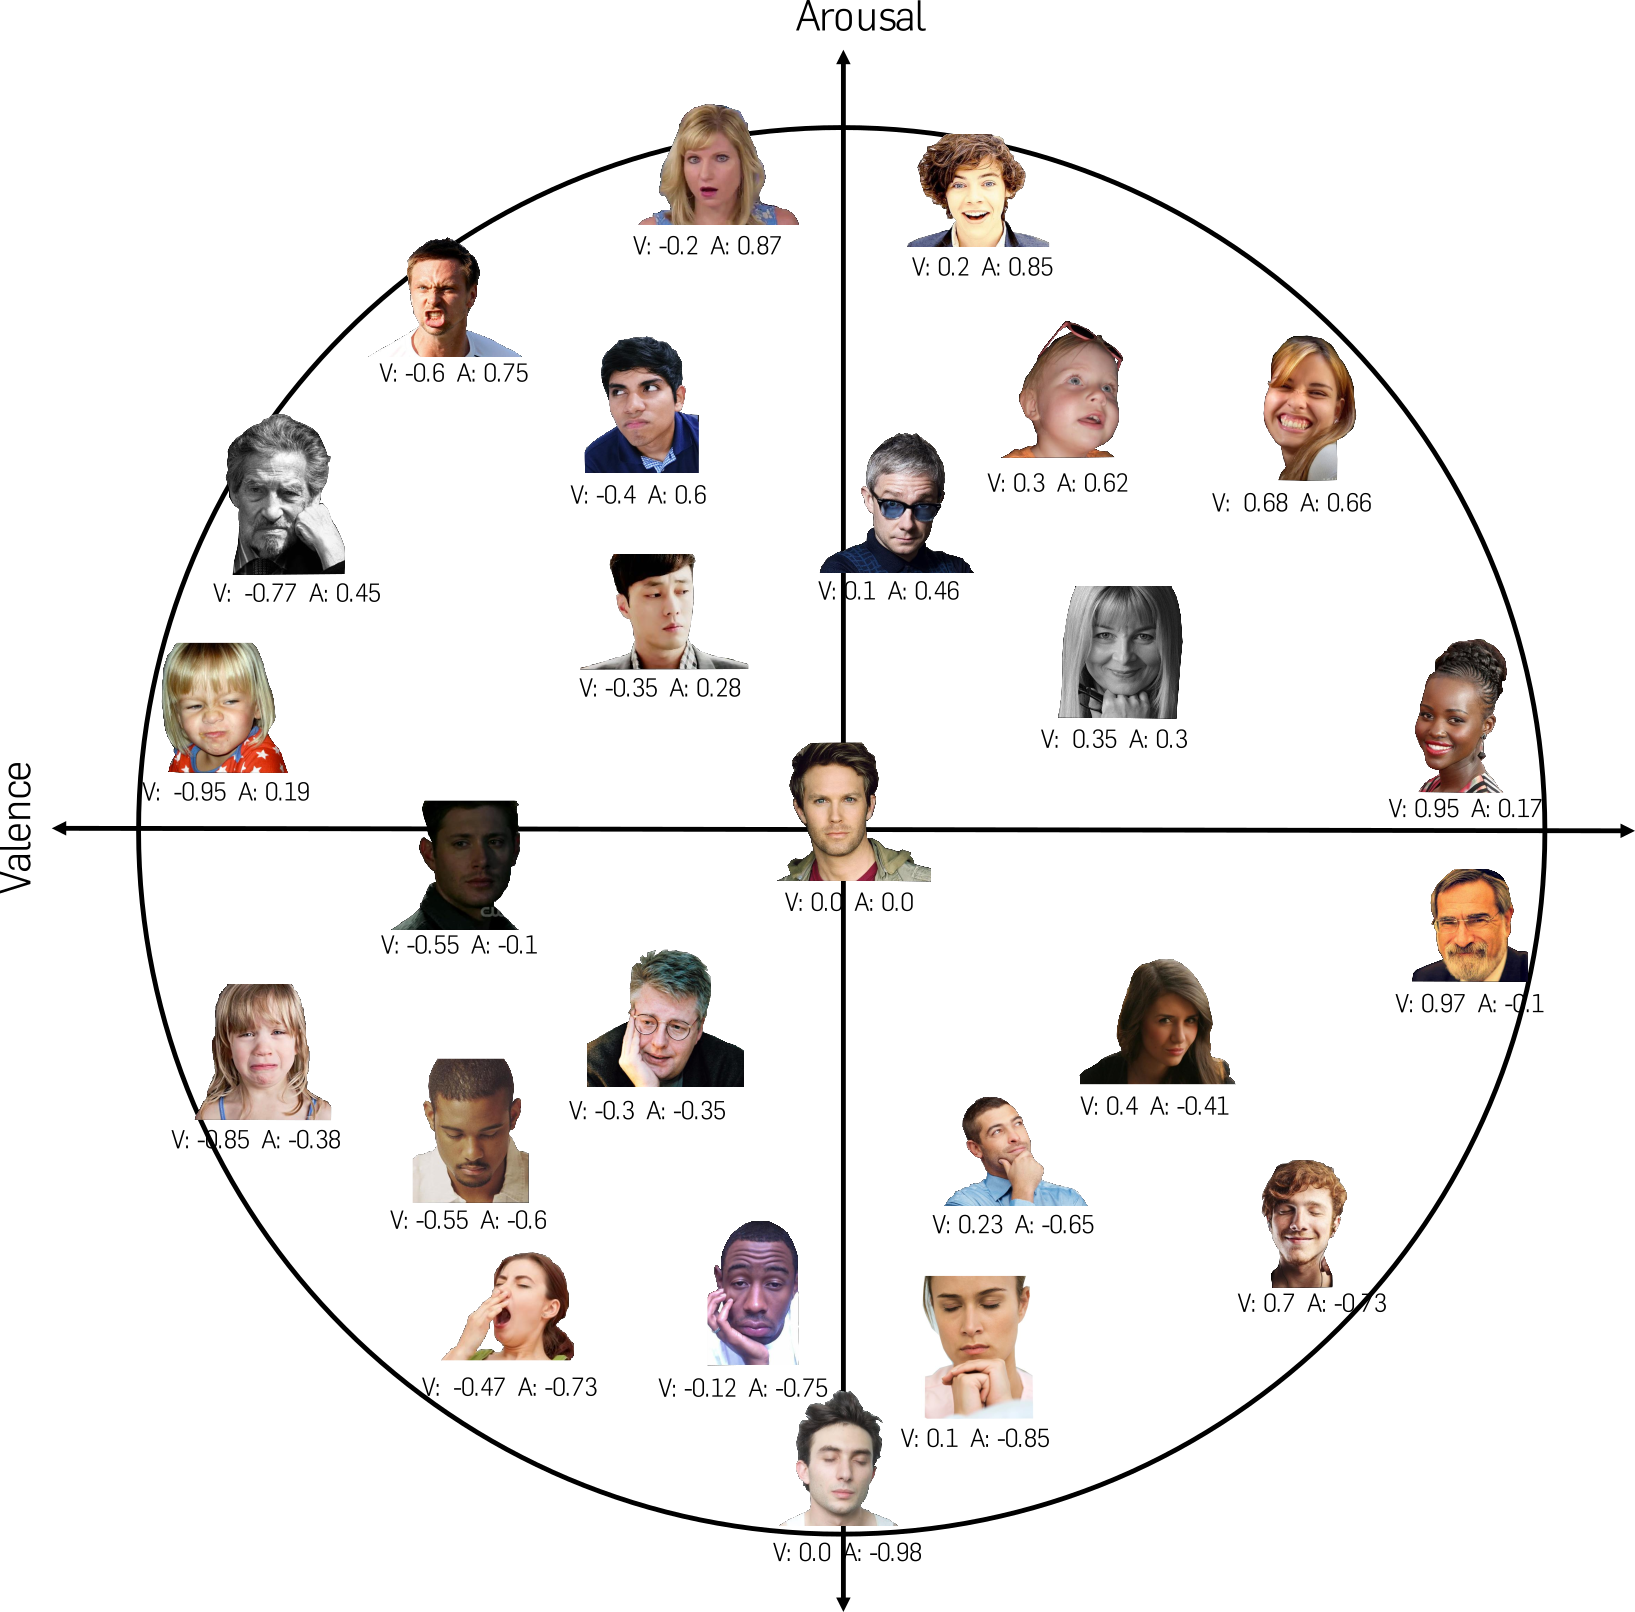
\includegraphics[width=0.65\linewidth]{AffectNet_circumplex.png}
    \end{center}
\end{frame}
}


\begin{frame}{P-A-D model}

By Albert Mehrabian and James A. Russell (1974)

Three-dimensional representation of emotion.

\begin{itemize}

\item \textbf{Pleasure, Arousal and Dominance}.
\item Most used model in robotics and Human-Machine Interaction
\end{itemize}

\pause

\textbf{Pleasure}: how pleasant is an emotion. Anger and fear are
unpleasant emotions, and score low on the pleasure scale. Joy is a
pleasant emotion.

\pause

\textbf{Arousal}: intensity of an emotion. Anger and rage are unpleasant
emotions, but rage has a higher intensity or a higher arousal state.
However boredom, which is also an unpleasant state, has a low arousal
value.

\pause

\textbf{Dominance}: controlling and dominant nature of the emotion. For
instance while both fear and anger are unpleasant emotions, anger is a
dominant emotion, while fear is a submissive emotion.

\end{frame}

{
    \paper{H. Hoffmann, A Scheck, T. Schuster, H. Kessler {\bf Mapping discrete
    emotions into the dimensional space: An empirical approach} 2012}
\begin{frame}{PAD model}

    \begin{columns}
        \begin{column}{0.5\linewidth}
    \begin{center}
        
\includegraphics[width=\linewidth]{pad}
    \end{center}


        \end{column}
        \begin{column}{0.5\linewidth}
        \begin{center}
            
\includegraphics[width=\linewidth]{pad-mapping}
        \end{center}
        \end{column}
    \end{columns}

\end{frame}
}

\miniframesoff

\begin{frame}[plain]
    \begin{center}
        Now, how to map automatically a face onto one of these models?
    \end{center}
\end{frame}

\miniframeson
%%%%%%%%%%%%%%%%%%%%%%%%%%%%%%%%%%%%%%%%%%%%%%%%%%%%%%%%%%%%%%%%%%%%%%%%%%%%%%%%%%%%%%
%%%%%%%%%%%%%%%%%%%%%%%%%%%%%%%%%%%%%%%%%%%%%%%%%%%%%%%%%%%%%%%%%%%%%%%%%%%%%%%%%%%%%%
%%%%%%%%%%%%%%%%%%%%%%%%%%%%%%%%%%%%%%%%%%%%%%%%%%%%%%%%%%%%%%%%%%%%%%%%%%%%%%%%%%%%%%

\section{Action Units}

\newcommand{\au}[1]{
    \includegraphics[width=2cm]{au/au-0#1.jpg}
}


{
    \paper{Ekman, {\bf The Facial Action Coding System}, 1977}
\begin{frame}{Facial Action Coding System}

    \begin{center}
         The {\bf Facial Action Coding System} (FACS) aim is to {\bf taxonomize
         human facial movements} by their appearance on the face.

        Facial movements are encoded as {\bf action units}.

    \end{center}

    \href{https://en.wikipedia.org/wiki/Facial_Action_Coding_System}{Wikipedia
    has a large list of action units}.
\end{frame}
}

{
    \paper{\source{https://www.cs.cmu.edu/\%7Eface/facs.htm}{Automated Face Analysis group, CMU}}
\begin{frame}{Action Units}
    \begin{center}

    \scriptsize
        \begin{tabular}{@{}p{0.5cm}p{2.5cm}p{3.5cm}p{2.5cm}@{}}
    \toprule
    \textbf{AU} & \textbf{Description} & \textbf{Facial muscle}                                                                   & \textbf{Example image} \\
    \midrule
    \only<1>{
    \textbf{1}  & Inner Brow Raiser    & \textit{Frontalis, pars medialis}                                                        & \au{01}                       \\
    \textbf{2}  & Outer Brow Raiser    & \textit{Frontalis, pars lateralis}                                                       & \au{02}                       \\
    \textbf{4}  & Brow Lowerer         & \textit{Corrugator supercilii, Depressor supercilii}                                     & \au{04}                       \\
    \textbf{5}  & Upper Lid Raiser     & \textit{Levator palpebrae superioris}                                                    & \au{05}                       \\
    \textbf{6}  & Cheek Raiser         & \textit{Orbicularis oculi, pars orbitalis}                                               & \au{06}                       \\
    \bottomrule
    }
    \only<2>{
    \textbf{7}  & Lid Tightener        & \textit{Orbicularis oculi, pars palpebralis}                                             & \au{07}                       \\
    \textbf{9}  & Nose Wrinkler        & \textit{Levator labii superioris alaquae nasi}                                           & \au{09}                       \\
    \textbf{10} & Upper Lip Raiser     & \textit{Levator labii superioris}                                                        & \au{10}                       \\
    \textbf{11} & Nasolabial Deepener  & \textit{Zygomaticus minor}                                                               & \au{11}                       \\
    \textbf{12} & Lip Corner Puller    & \textit{Zygomaticus major}                                                               & \au{12}                       \\
    \bottomrule
    }
    \only<3>{
    \textbf{13} & Cheek Puffer         & \textit{Levator anguli oris (a.k.a. Caninus)}                                            & \au{13}                       \\
    \textbf{14} & Dimpler              & \textit{Buccinator}                                                                      & \au{14}                       \\
    \textbf{15} & Lip Corner Depressor & \textit{Depressor anguli oris (a.k.a. Triangularis)}                                     & \au{15}                       \\
    \textbf{16} & Lower Lip Depressor  & \textit{Depressor labii inferioris}                                                      & \au{16}                       \\
    \bottomrule
    }
    \only<4>{
    \textbf{17} & Chin Raiser          & \textit{Mentalis}                                                                        & \au{17}                       \\
    \textbf{18} & Lip Puckerer         & \textit{Incisivii labii superioris and Incisivii labii inferioris}                       & \au{18}                       \\
    \textbf{20} & Lip stretcher        & \textit{Risorius w/ platysma}                                                            & \au{20}                       \\
    \textbf{22} & Lip Funneler         & \textit{Orbicularis oris}                                                                & \au{22}                       \\
    \textbf{23} & Lip Tightener        & \textit{Orbicularis oris}                                                                & \au{23}                       \\
    \bottomrule
    }
    \only<5>{
    \textbf{24} & Lip Pressor          & \textit{Orbicularis oris}                                                                & \au{24}                       \\
    \textbf{25} & Lips part            & \textit{Depressor labii inferioris or relaxation of Mentalis, or Orbicularis oris}       & \au{25}                       \\
    \textbf{26} & Jaw Drop             & \textit{Masseter, relaxed Temporalis and internal Pterygoid}                             & \au{26}                       \\
    \textbf{27} & Mouth Stretch        & \textit{Pterygoids, Digastric}                                                           & \au{27}                       \\
    \bottomrule
    }
    \only<6>{
    \textbf{28} & Lip Suck             & \textit{Orbicularis oris}                                                                & \au{28}                       \\
    \textbf{41} & Lid droop            & \textit{Relaxation of Levator palpebrae superioris}                                      & \au{41}                       \\
    \textbf{42} & Slit                 & \textit{Orbicularis oculi}                                                               & \au{42}                       \\
    \textbf{43} & Eyes Closed          & \textit{Relaxation of Levator palpebrae superioris; Orbicularis oculi, pars palpebralis} & \au{43}                       \\
    \textbf{44} & Squint               & \textit{Orbicularis oculi, pars palpebralis}                                             & \au{44}                       \\
    \bottomrule
    }
    \only<7>{
    \textbf{45} & Blink                & \textit{Levator palpebrae superioris; Orbicularis oculi, pars palpebralis} &                               \\
    \textbf{46} & Wink                 & \textit{Levator palpebrae superioris; Orbicularis oculi, pars palpebralis} &                               \\
    \textbf{51} & Head turn left       &                                                                                          & \au{51}                       \\
    \textbf{52} & Head turn right      &                                                                                          & \au{52}                       \\
    \bottomrule
    }
    \only<8>{
    \textbf{53} & Head up              &                                                                                          & \au{53}                       \\
    \textbf{54} & Head down            &                                                                                          & \au{54}                       \\
    %\textbf{55} & Head tilt left       &                                                                                          & \au{55}                       \\
    %\textbf{56} & Head tilt right      &                                                                                          & \au{56}                       \\
    \bottomrule
    }
    \only<9>{
    %\textbf{57} & Head forward         &                                                                                          & \au{57}                       \\
    %\textbf{58} & Head back            &                                                                                          & \au{58}                       \\
    \textbf{61} & Eyes turn left       &                                                                                          & \au{61}                       \\
    \textbf{62} & Eyes turn right      &                                                                                          & \au{62}                       \\
    \textbf{63} & Eyes up              &                                                                                          & \au{63}                       \\
    \textbf{64} & Eyes down            &                                                                                          & \au{64}                       \\ 
    \bottomrule
    }
    \end{tabular}
    \end{center}

\end{frame}
}

\begin{frame}{OpenFace Action Units}
    \begin{center}
        OpenFace is an open-source library that recognises 17 action units.

        \href{https://github.com/TadasBaltrusaitis/OpenFace}{github.com/TadasBaltrusaitis/OpenFace}
        \vspace{2em}

        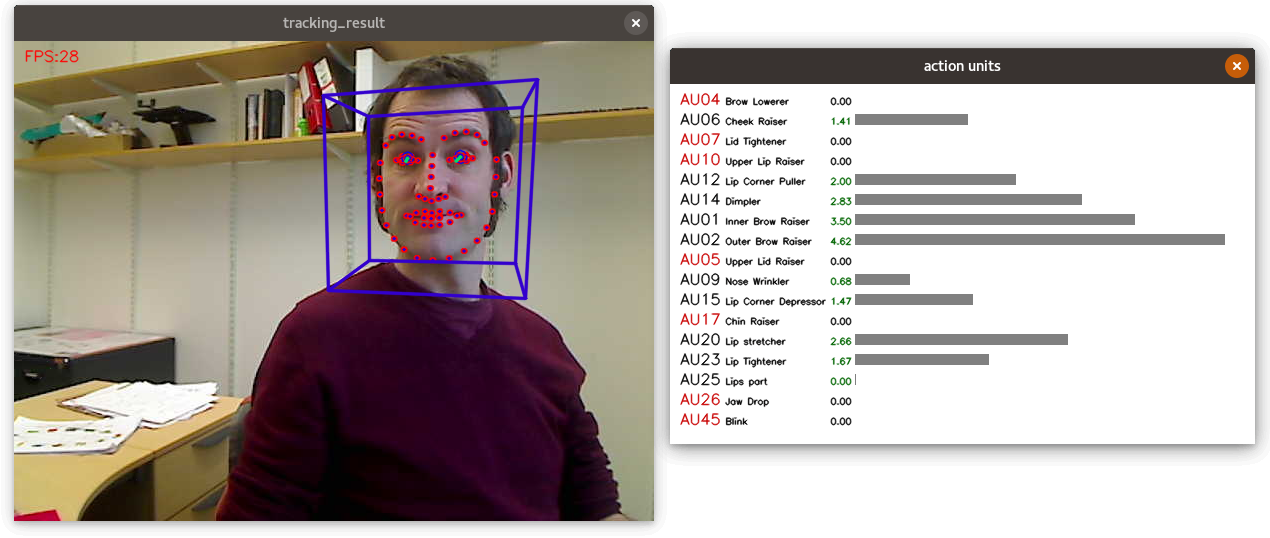
\includegraphics[width=0.9\linewidth]{au-openface}

        \scriptsize
        (not to be confused with this other \href{https://github.com/cmusatyalab/openface}{CMU OpenFace})
    \end{center}
\end{frame}

\begin{frame}{OpenFace 17 Action Units}

    \begin{columns}
        \begin{column}{0.5\linewidth}
    \begin{center}

    \scriptsize
        \begin{tabular}{@{}p{0.3cm}p{2.5cm}p{2cm}@{}}
    \toprule
    \textbf{AU} & \textbf{Description} & \textbf{Example image} \\
    \midrule
    \only<1>{
    \textbf{1}  & Inner Brow Raiser    &  \au{01} \\
    \textbf{2}  & Outer Brow Raiser    &  \au{02} \\
    \textbf{4}  & Brow Lowerer         &  \au{04} \\
    \textbf{5}  & Upper Lid Raiser     &  \au{05} \\
    \textbf{6}  & Cheek Raiser         &  \au{06} \\
    \bottomrule
    }
    \only<2>{
    \textbf{15} & Lip Corner Depressor &  \au{15} \\
    \textbf{17} & Chin Raiser          &  \au{17} \\
    \textbf{20} & Lip stretcher        &  \au{20} \\
    \textbf{23} & Lip Tightener        &  \au{23} \\
    \bottomrule
    }
    \end{tabular}
    \end{center}
            
        \end{column}
        \begin{column}{0.5\linewidth}
    \begin{center}

    \scriptsize
        \begin{tabular}{@{}p{0.3cm}p{2cm}p{2cm}@{}}
    \toprule
    \textbf{AU} & \textbf{Description} & \textbf{Example image} \\
    \midrule
    \only<1>{
    \textbf{7}  & Lid Tightener        &  \au{07} \\
    \textbf{9}  & Nose Wrinkler        &  \au{09} \\
    \textbf{10} & Upper Lip Raiser     &  \au{10} \\
    \textbf{12} & Lip Corner Puller    &  \au{12} \\
    \bottomrule
    }
    \only<2>{
    \textbf{14} & Dimpler              &  \au{14} \\
    \textbf{25} & Lips part            &  \au{25} \\
    \textbf{26} & Jaw Drop             &  \au{26} \\
    \textbf{45} & Blink                &          \\
    \bottomrule
    }
    \end{tabular}
    \end{center}
         \end{column}
    \end{columns}

\end{frame}


\section[Emotion classifier]{Let's build our own emotion classifier from scratch}

\begin{frame}{Shopping list}

    \begin{center}
        {\bf What do we need?}
    \end{center}

    \pause

    \begin{itemize}
        \item<+-> a dataset of labelled faces
        \item<+-> some pre-processing faces to normalise them
        \item<+-> features to extract
        \item<+-> a classifier
    \end{itemize}
\end{frame}

\imageframe[color=black]{google-emotions-query}
\imageframe[color=black]{emotions_dataset}
\imageframe[color=black]{emotions_dataset_aligned}
\imageframe[color=black]{emotion-dataset-csv}

\begin{frame}{Our tiny 'emotions' dataset}
    \begin{itemize}
        \item A couple of \href{https://www.google.co.uk/search?q=human+face+happiness&tbm=isch&source=lnt&tbs=itp:face}{Google queries}
        \item a bit of manual filtering
        \item 558 faces, between 70 and 130 per emotion
        \item split into 2 datasets: a {\bf training} dataset (50 face per
            emotion) and a {\bf testing} dataset
        \item for each face, OpenFace pre-processing to:
            \begin{itemize}
                \item extract facial landmarks
                \item normalise and mask out the faces
                \item extract action units
            \end{itemize}
    \end{itemize}

    The dataset is available for you to play with on the lecture's
    \href{https://github.com/severin-lemaignan/lecture-hri-emotions}{GitHub repo}.
\end{frame}

\begin{frame}{Classification?}

    We want to train a classifier with our training dataset, and then check
    whether the emotions in the test faces can be properly recognised.

    \begin{center}
        {\bf What are our options here?}
    \end{center}

    \pause

    \begin{enumerate}
        \item<+-> 'eigenfaces' (PCA) on the training dataset; then project test
            faces +
            kNN/SVM (\ie face recognition with 6 possible classes)
        \item<+-> LDA instead of PCA to improve inter-class discrimination
        \item<+-> kNN/SVM on the action units directly?
        \item<+-> PCA, then kNN/SVM on the action units?
        \item<+-> LDA, then kNN/SVM on the action units?
    \end{enumerate}
\end{frame}

\begin{frame}[fragile]{Python helpers}
\begin{pythoncode}
import numpy as np
import PIL.Image as Image
import matplotlib.pyplot as plt

def read_image(path):
    im = Image.open(path)
    im = im.convert("L") # to grayscale
    return np.asarray(im, dtype=np.uint8).flatten()

def plot_embedding(X, labels):

    x_min, x_max = np.min(X, 0), np.max(X, 0)
    X = (X - x_min) / (x_max - x_min)

    plt.figure()
    ax = plt.subplot(111)
    for i in range(X.shape[0]):
        plt.text(X[i, 0], X[i, 1], str(labels[i])],
                 color=plt.cm.Dark2((int(labels[i]) + 1) / 8.))
\end{pythoncode}
\end{frame}


\begin{frame}[fragile]{PCA on the dataset}
    \begin{pythoncode}
import csv
from sklearn.decomposition import PCA

training_images = []
training_categories = []
with open("training.csv", 'r') as csvfile:
    details = csv.DictReader(csvfile, skipinitialspace=True)
    for row in details:
        training_images.append(read_image(row["face"]))
        training_categories.append(row["emotion"])

# same for testing set
testing_images = ...
testing_categories = ...

pca = PCA(n_components=20)
pca.fit(training_images)

# plots only the 2 first coordinates in PCA space
plot_embedding(pca.transform(training_images), training_categories)
plot_embedding(pca.transform(testing_images), testing_categories)

\end{pythoncode}
\end{frame}

\imageframe{image_pca_train}
\imageframe{image_pca_test}
\begin{frame}{Classification results, PCA}
    \% of successful emotion prediction out of 258 test faces

    {\bf kNN}:
    \begin{itemize}
        \item k=1: 30.2\%
        \item k=2: 26.0\%
        \item k=4: 28.3\%
        \item k=6: 30.2\%
        \item k=9: 33.7\%
    \end{itemize}

    {\bf SVM}:

    \begin{itemize}
            \item kernel: rbf: 19.4\%
    \end{itemize}
\end{frame}

\begin{frame}[fragile]{LDA on the dataset}
    \begin{pythoncode}
from sklearn.discriminant_analysis import LinearDiscriminantAnalysis

lda = LinearDiscriminantAnalysis(n_components=20)

lda.fit(training_images, training_categories)

plot_embedding(lda.transform(training_images), training_categories)
plot_embedding(lda.transform(testing_images), testing_categories)
\end{pythoncode}
\end{frame}


\imageframe{image_lda_train}

\begin{frame}{Linear Discriminant Analysis overfitting}

    \begin{center}
        Great result? No! Massive overfitting!
    \end{center}

    LDA requires the number of samples per class $n$ (\ie number of faces per
    emotion, 50 here) to be much larger than the number of features $p$ (in our case,
    $112\times 112$ px $= 12544$!)

    Rule of thumb: $n > 3\cdot p$

    ...not going to work if we use the pixels directly.
\end{frame}

\imageframe{image_lda_test}

\begin{frame}{}

    {\bf Idea}: first, reduce dimensionality (using PCA for instance), and then,
    perform a LDA on the lower dimensionality representation.
\end{frame}


\begin{frame}[fragile]{PCA + LDA on the dataset}
    \begin{pythoncode}
from sklearn.decomposition import PCA
from sklearn.discriminant_analysis import LinearDiscriminantAnalysis

# first, PCA on 12544-D observations
pca = PCA(n_components=20)
pca.fit(training_images)

# then LDA on 20-D observations
lda = LinearDiscriminantAnalysis(n_components=10)
lda.fit(pca.transform(training_images), training_categories)

# apply the transform...
lda_pca_training_images = lda.transform(pca.transform(training_images))
lda_pca_testing_images = lda.transform(pca.transform(testing_images))

# and plot!
plot_embedding(lda_pca_training_images, training_categories)
plot_embedding(lda_pca_testing_images, testing_categories)
\end{pythoncode}
\end{frame}


\imageframe{image_pca_lda_train}
\imageframe{image_pca_lda_test}

\begin{frame}{Classification results, PCA followed with LDA}
    \% of successful emotion prediction out of 258 test faces

    {\bf kNN}:
    \begin{itemize}
        \item k=1: 39.5\%
        \item k=2: 33.3\%
        \item k=4: 36.4\%
        \item k=6: 35.7\%
        \item k=9: 36.8\%
    \end{itemize}

    {\bf SVM}:

    \begin{itemize}
        \item kernel: rbf: 41.9\%
        \item kernel: linear: 38.4\%
        \item kernel: poly: 26.0\%
    \end{itemize}
\end{frame}

\begin{frame}{Confusion matrix}
    \begin{center}
        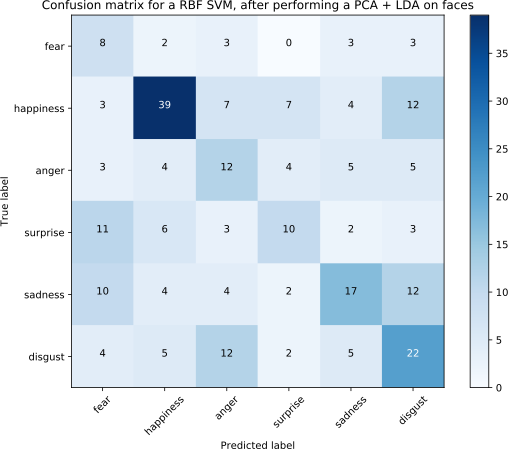
\includegraphics[width=0.8\linewidth]{confusion_matrix_image_pca_lda_svm}
    \end{center}
\end{frame}

\begin{frame}[fragile]{Classification results, Action Units}
    

    \begin{center}
        {\bf What about classifying using the 17 action units directly?}
    \end{center}

    \begin{columns}
        \begin{column}{0.4\linewidth}
    {\bf kNN}:
    \begin{itemize}
        \item k=1: 46.9\%
        \item k=2: 42.2\%
        \item k=4: 50.8\%
        \item k=6: 46.1\%
        \item k=9: 52.3\%
    \end{itemize}

    {\bf SVM}:

    \begin{itemize}
        \item kernel: rbf: 48.8\%
        \item kernel: linear: 52.3\%
        \item kernel: poly: 38.0\%
    \end{itemize}

        \end{column}
        \begin{column}{0.6\linewidth}
            \begin{pythoncode}
from numpy import genfromtxt
from sklearn import neighbors, svm

csv_train = genfromtxt('training.csv')
training = csv_train[:,1:-1]
training_categories = csv_train[:,0]

csv_test = genfromtxt('testing.csv')
testing = csv_test[:,1:-1]
testing_categories = csv_test[:,0]

clf = neighbors.KNeighborsClassifier(k)
clf.fit(training, training_categories)
knns_predictions = clf.predict(testing)

clf = svm.SVC(kernel=kernel)
clf.fit(training, training_categories)
svm_predictions = clf.predict(testing)

            \end{pythoncode}
        \end{column}
    \end{columns}

\end{frame}


\imageframe{au_pca_train}
\imageframe{au_pca_test}
\begin{frame}{Classification results, PCA  on AUs}

    Classification on the first 5 eigen components.

    {\bf kNN}:
    \begin{itemize}
        \item k=1: 45.7\%
        \item k=2: 39.1\%
        \item k=4: 45.0\%
        \item k=6: 43.8\%
        \item k=9: 47.3\%
    \end{itemize}

    {\bf SVM}:

    \begin{itemize}
        \item kernel: rbf: 50.8\%
        \item kernel: linear: 47.7\%
        \item kernel: poly: 39.9\%
    \end{itemize}

    $\Rightarrow$ no improvement
\end{frame}

\imageframe{au_lda_train}
\imageframe{au_lda_test}
\begin{frame}{Classification results, LDA  on AUs}

    \only<1>{
    Classification on the first 5 components.


    {\bf kNN}:
    \begin{itemize}
        \item k=1: 45.7\%
        \item k=2: 43.0\%
        \item k=4: 45.7\%
        \item k=6: 46.9\%
        \item k=9: 52.3\%
    \end{itemize}

    {\bf SVM}:

    \begin{itemize}
        \item kernel: rbf: 53.1\%
        \item kernel: linear: 51.9\%
        \item kernel: poly: 40.3\%
    \end{itemize}

    $\Rightarrow$ same as direct, better than PCA
    }

    \only<2>{
        With only {\bf 2 components}:

    {\bf kNN}:
    \begin{itemize}
        \item k=1: 43.4\%
        \item k=2: 42.6\%
        \item k=4: 49.2\%
        \item k=6: 51.2\%
        \item k=9: 49.2\%
    \end{itemize}

    {\bf SVM}:

    \begin{itemize}
        \item kernel: rbf: 53.9\%
        \item kernel: linear: 48.8\%
        \item kernel: poly: 39.9\%
    \end{itemize}

    $\Rightarrow$ {\bf 2 values, extracted from the faces, are sufficient to
    recognise an emotion $\approx 54$\% of the time.}
    }

\end{frame}

\begin{frame}{Confusion matrix}
    \begin{center}
        \includegraphics<1>[width=0.8\linewidth]{confusion_matrix_au_lda_svm}

        \includegraphics<2>[width=0.45\linewidth]{confusion_matrix_au_lda_svm}
        \includegraphics<2>[width=0.45\linewidth]{confusion_matrix_image_pca_lda_svm}
    \end{center}
\end{frame}


\begin{frame}{How to improve it further?}

    \begin{center}
        Ideas?
    \end{center}

    \pause

    \begin{itemize}
        \item better dataset (wider range of facial expressions)
        \item larger dataset
        \item use the facial landmark directly?
        \item different classifier $\rightarrow$ neural network (deep or not)?
    \end{itemize}

\end{frame}

\imageframe[color=black,caption=Natural emotions are much harder]{natural-emotions-hulot}

\section[Generation]{Generating emotional responses}

\imageframe{wall-e}

\begin{frame}{How to express the robot's internal state?}
    \begin{itemize}
        \item facial expressions (when available!)
        \item Gestures/postures
        \item non-verbal utterances, sounds
        \item dynamics of motion
        \item proxemics
        \item ...
    \end{itemize}
\end{frame}


\begin{frame}{How expressive a robot can be?}

    \begin{columns}
        \begin{column}{0.5\linewidth}
            \begin{center}
                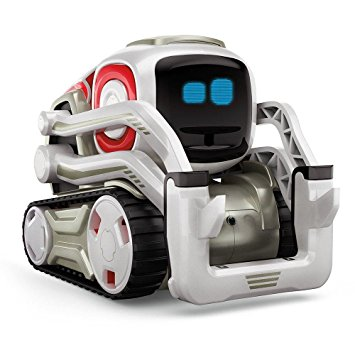
\includegraphics[width=0.8\linewidth]{cozmo}
            \end{center}
        \end{column}
        \begin{column}{0.5\linewidth}
            \href{https://www.anki.com/en-gb/cozmo}{Anki's Cozmo}
        \end{column}
    \end{columns}
\end{frame}

\videoframe[0.56]{figs/cozmo.mp4}

\imageframe[color=black]{cozmo-expression-sheet}

\videoframe[0.56]{figs/readability.m4v}
\videoframe{figs/nlu-starwars.mp4}
\videoframe[0.56]{figs/nlu.mp4}

\section{Anthropomorphism}

\imageframe[footnote=Source: Christoph Bartneck,scale=0.9]{bartneck}

\imageframe{anthropo}

\begin{frame}{Dynamics of anthropomorphism}
    \begin{center}
        \includegraphics<1>[width=0.8\linewidth]{dynamics-0}
        \includegraphics<2>[width=0.8\linewidth]{dynamics-1}
        \includegraphics<3>[width=0.8\linewidth]{dynamics-2}
        \includegraphics<4>[width=0.8\linewidth]{dynamics-3}
    \end{center}
\end{frame}

\begin{frame}{Cozmo?}

    \begin{columns}
        \begin{column}{0.4\linewidth}
            \begin{center}
                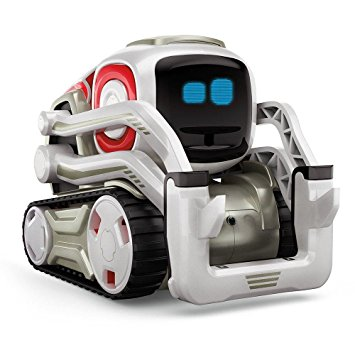
\includegraphics[width=0.8\linewidth]{cozmo}
            \end{center}
        \end{column}
        \begin{column}{0.6\linewidth}
            \begin{center}
                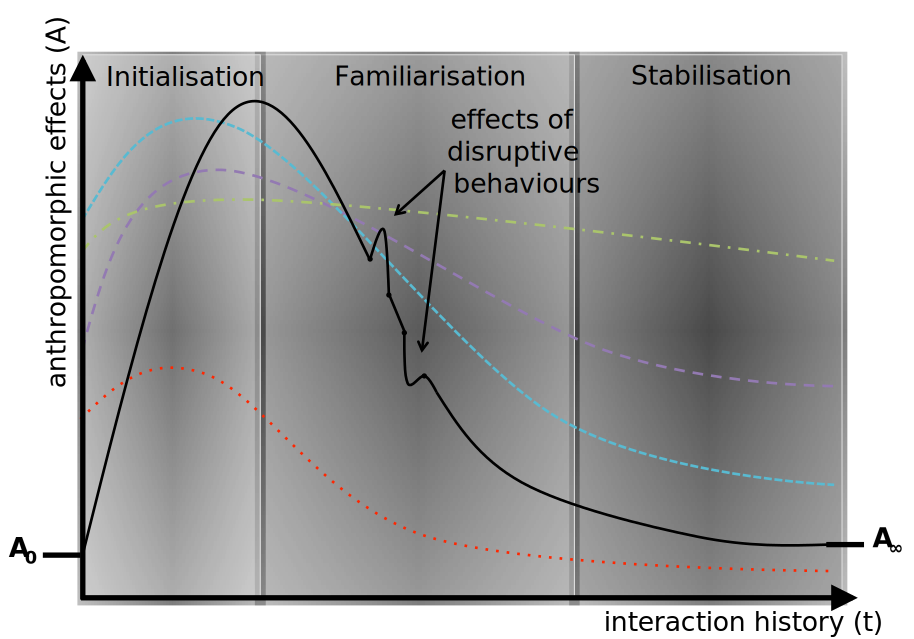
\includegraphics[width=\linewidth]{dynamics-3}
            \end{center}
        \end{column}
    \end{columns}
\end{frame}


\begin{frame}{Disruptive behaviours to elicit engagement?}
    \begin{columns}
        \begin{column}{0.5\linewidth}
            \begin{center}
            \video[0.56]{0.9\linewidth}{figs/ranger/correct.mp4}

            \video[0.56]{0.9\linewidth}{figs/ranger/mistake.mp4}
            \end{center}
        \end{column}
        \begin{column}{0.5\linewidth}
            \begin{center}
            \video[0.56]{0.9\linewidth}{figs/ranger/lost.mp4}

            \video[0.56]{0.9\linewidth}{figs/ranger/disobey.mp4}
            \end{center}
        \end{column}
    \end{columns}
\end{frame}

{
    \paper{Lemaignan, Fink, Mondada, Dillenbourg {\bf You're Doing
    It Wrong! Studying Unexpected Behaviors in CRI} ICSR
    2015}
\fullbackground{ranger/ranger-background}

\begin{frame}{Anthropomorphism != Engagement}

    \begin{figure}
        \hspace*{5cm}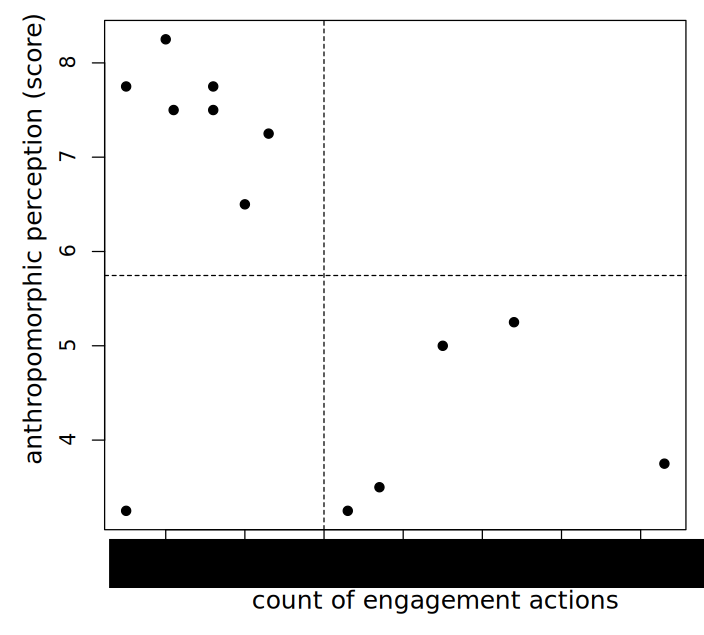
\includegraphics[width=0.6\linewidth]{ranger/domino-correlation}
    \end{figure}

\end{frame}
}


\miniframesoff

\begin{frame}{}
    \begin{center}
        \Large
        That's all for today, folks!\\[2em]
        \normalsize
        Questions:\\
        Portland Square B316 or \url{severin.lemaignan@plymouth.ac.uk} \\[1em]

        Slides:\\
        \href{https://github.com/severin-lemaignan/lecture-emotions}{\small
        github.com/severin-lemaignan/lecture-emotions}

    \end{center}
\end{frame}




\end{document}
